\documentclass[10pt,twocolumn]{article}
\usepackage[margin=0.75in]{geometry}
\usepackage{amsmath,amssymb,amsthm}
\usepackage{booktabs}
\usepackage{graphicx}
\usepackage{hyperref}
\usepackage{url}
\usepackage{xcolor}
\usepackage{algorithm}
\usepackage{algpseudocode}
\usepackage{microtype}
\usepackage{caption}
\usepackage{subcaption}
\usepackage{tikz}
\usepackage{pgfplots}
\pgfplotsset{compat=1.18}

\hypersetup{
    colorlinks=true,
    linkcolor=blue,
    citecolor=blue,
    urlcolor=blue
}

\newcommand{\bm}[1]{\boldsymbol{#1}}
\newcommand{\Eop}{\mathbb{E}}
\newcommand{\R}{\mathbb{R}}
\newcommand{\cO}{\mathcal{O}}

\title{\textbf{TurboQuant+: Near-Lossless KV Cache Compression\\
with 3-bit Value Quantization for Long-Context LLM Inference}}

\author{
  Themo (arun.rajendra8@gmail.com)\\
  \textit{Independent Research}\\
  \and
  Contributions to: \texttt{github.com/0xSero/turboquant}
}

\date{April 2026}

\begin{document}

\maketitle

\begin{abstract}
KV cache memory is the primary bottleneck for long-context LLM inference, growing linearly with sequence length. TurboQuant addresses this via random orthogonal rotation combined with Lloyd-Max scalar quantization for keys and asymmetric group quantization for values, achieving approximately 4--5$\times$ compression. In this work, we systematically characterize TurboQuant's quality-compression tradeoffs and contribute two practical improvements. First, reducing the value quantization group size from 32 to 16 improves cosine similarity from 0.932 to 0.952 at zero compression cost—a one-line default change. Second, implementing true 3-bit value packing (8 values per 3 bytes) raises cosine similarity to 0.987, approaching 4-bit quality (0.997) at only 33\% more storage than 2-bit. We validate all three Triton fused decode kernels on an NVIDIA RTX A4000, confirming numerical correctness to floating-point precision and measuring 20--60$\times$ decode speedup over PyTorch at 4k--16k context lengths. We further demonstrate that the Randomized Hadamard Transform (RHT) is quality-equivalent to the stored QR rotation matrix ($< 0.001$ cosine difference) while requiring 102$\times$ less memory for $d = 128$. Finally, we provide a context capacity analysis showing that 3-bit keys with 2-bit values enables 2.39 million tokens in 16.8 GB VRAM—a 3.88$\times$ extension over FP16. All improvements have been contributed back to the open-source TurboQuant repository.
\end{abstract}

\textbf{Keywords:} KV cache compression, LLM inference, quantization, Triton kernels, long-context inference, Hadamard transform

%---------------------------------------------------------------------
\section{Introduction}
\label{sec:intro}
%---------------------------------------------------------------------

Transformer-based large language models (LLMs) require storing all past key-value (KV) activations during autoregressive generation. This KV cache grows linearly with sequence length, number of heads, and layers: for a 32-head, dimension-128 model in FP16, each token consumes $32 \times 128 \times 2 \times 2 = 16{,}384$ bytes. An NVIDIA RTX A4000 with 16.8 GB VRAM can hold approximately 615k tokens at FP16 precision—insufficient for emerging 1M+ context applications~\cite{liu2023longrange}.

KV cache compression has emerged as the dominant approach to this bottleneck. Existing methods broadly fall into three categories: (1) \emph{eviction-based} methods~\cite{zhang2023h2o} that drop low-importance tokens, (2) \emph{quantization-based} methods~\cite{liu2024kivi,hooper2024kvquant} that reduce per-token bit-width, and (3) \emph{hybrid} approaches that combine both. Quantization-based methods are particularly attractive because they are lossless in the information-theoretic sense—they preserve all tokens while trading reconstruction fidelity for memory.

TurboQuant~\cite{turboquant2025} represents a theoretically principled approach: it combines random orthogonal rotation with Lloyd-Max optimal scalar quantization for keys, and QJL (Quantized Johnson-Lindenstrauss) projections to produce \emph{provably unbiased} attention score estimates. This unbiasedness property—that $\Eop[\hat{s}] = s$ for the estimated attention score $\hat{s}$ and true score $s$—is a stronger guarantee than reconstruction fidelity alone. However, TurboQuant's default 2-bit value quantization introduces a measurable quality gap (cosine similarity 0.932 vs 1.0 for FP16), which can limit output quality for generation tasks.

\subsection*{Contributions}
This paper makes the following contributions:

\begin{enumerate}
\item \textbf{Group size analysis}: We show that reducing value quantization group size from 32 to 16 yields $+0.020$ cosine similarity improvement at zero compression cost. This is the single most impactful free improvement available (Section~\ref{sec:value_quant}).

\item \textbf{True 3-bit value quantization}: We design and implement a true 3-bit packing scheme (8 values per 3 bytes) that raises value reconstruction cosine similarity from 0.932 to 0.987—approaching 4-bit quality at 1.33$\times$ the bytes of 2-bit (Section~\ref{sec:3bit}).

\item \textbf{Triton kernel validation}: We independently validate all three Triton fused decode kernels on GPU hardware, confirming correctness to floating-point precision and measuring 20--60$\times$ speedup over the PyTorch fallback path (Section~\ref{sec:kernels}).

\item \textbf{RHT quality equivalence}: We prove empirically that the Randomized Hadamard Transform (RHT) is quality-equivalent to QR rotation ($< 0.001$ cosine difference across all tested configurations) while requiring 102$\times$ less memory for $d = 128$ (Section~\ref{sec:rht}).

\item \textbf{Context capacity analysis}: We characterize achievable context lengths on commodity hardware, demonstrating 3.88$\times$ context extension vs FP16 on the RTX A4000 with 3-bit keys and 2-bit values (Section~\ref{sec:capacity}).
\end{enumerate}

%---------------------------------------------------------------------
\section{Background and Related Work}
\label{sec:background}
%---------------------------------------------------------------------

\subsection{KV Cache Compression}

\textbf{KIVI}~\cite{liu2024kivi} performs per-channel asymmetric 2-bit quantization of keys and values without fine-tuning, achieving 2-bit compression with minimal perplexity degradation. Unlike TurboQuant, KIVI does not use rotation to Gaussianize the distribution before quantization.

\textbf{KVQuant}~\cite{hooper2024kvquant} applies non-uniform quantization by learning per-channel codebooks from activation statistics, targeting 10M+ context lengths. It requires calibration data and per-layer codebook storage.

\textbf{H2O}~\cite{zhang2023h2o} takes an eviction approach: it identifies "heavy hitter" tokens (those with high cumulative attention scores) and evicts the rest. This introduces information loss but can be combined with quantization.

\textbf{FlashAttention}~\cite{dao2022flashattention} reduces memory bandwidth for \emph{computing} attention by tiling the softmax, but does not compress the stored KV cache itself.

\subsection{Quantization Theory}

\textbf{Lloyd-Max quantization}~\cite{lloyd1982least,max1960quantizing} provides the optimal scalar quantizer for a given distribution and bit-width, minimizing mean squared error. For Gaussian inputs with $d$ dimensions, after random orthogonal rotation, each coordinate is approximately Beta-distributed (bounded in $[-1, 1]$ due to normalization), making Lloyd-Max codebooks natural.

\textbf{Group quantization} reduces quantization granularity by computing independent scale and zero-point parameters per group of $G$ elements~\cite{frantar2023gptq}. Smaller $G$ reduces within-group variation and improves reconstruction quality at the cost of metadata overhead ($O(d/G)$ parameters per vector).

\subsection{Johnson-Lindenstrauss Projections}

The QJL (Quantized Johnson-Lindenstrauss) component of TurboQuant builds on the classic JL lemma~\cite{johnson1984extensions}: a random projection into $m$ dimensions approximately preserves inner products. TurboQuant uses 1-bit sign quantization of a random Gaussian projection to capture the residual error after MSE quantization, producing an unbiased estimator of the true attention score.

%---------------------------------------------------------------------
\section{TurboQuant Overview}
\label{sec:turboquant}
%---------------------------------------------------------------------

We briefly review TurboQuant's core algorithms to establish notation for our improvements.

\subsection{Key Quantization: TurboQuantMSE}

For a key vector $\bm{k} \in \R^d$ with $\|\bm{k}\| = 1$ (after normalization), TurboQuantMSE applies:

\begin{enumerate}
\item \textbf{Rotation}: $\tilde{\bm{k}} = \bm{k} \Pi^\top$ where $\Pi \in \R^{d \times d}$ is a random orthogonal matrix.
\item \textbf{Scalar quantization}: Each coordinate $\tilde{k}_i$ is quantized via Lloyd-Max codebook at $b$ bits.
\item \textbf{Bit-packing}: For $b = 3$, indices are packed at 2 values per byte (4-bit aligned).
\end{enumerate}

The stored representation is: packed indices $\hat{\bm{k}} \in \{0, \ldots, 2^b - 1\}^d$ and the scalar norm $\|\bm{k}\|$.

\subsection{Attention Score Estimation: TurboQuantProd}

For query $\bm{q} \in \R^d$ and compressed key $(\hat{\bm{k}}, \|\bm{k}\|)$, TurboQuantProd computes:

$$\hat{s} = \hat{s}_\text{MSE} + \hat{s}_\text{QJL}$$

where $\hat{s}_\text{MSE}$ is the MSE-optimal estimate using $(b-1)$-bit quantization and $\hat{s}_\text{QJL}$ is a 1-bit QJL correction term. The combined estimator satisfies $\Eop[\hat{s}] = \langle \bm{q}, \bm{k} \rangle$, with variance that decreases with $N$ (the number of tokens, via self-normalization of softmax).

\subsection{Value Quantization}
\label{sec:value_overview}

Values are quantized via asymmetric per-group min-max quantization. For group $g$ of a value vector $\bm{v} \in \R^d$:

\begin{align}
\text{scale}_g &= \frac{\max(\bm{v}_g) - \min(\bm{v}_g)}{2^b - 1} \\
\bm{v}_g^{(q)} &= \text{round}\!\left(\frac{\bm{v}_g - \min(\bm{v}_g)}{\text{scale}_g}\right)
\end{align}

The original TurboQuant default was $b = 2$, $G = 32$. Values are not rotated before quantization (unlike keys), so they receive no Gaussianization benefit and the 2-bit reconstruction quality (cosine similarity 0.932) is the primary quality bottleneck.

\subsection{Triton Fused Decode Kernels}

TurboQuant ships three Triton kernels:
\begin{itemize}
\item \textbf{Kernel 1} (\texttt{turboquant\_mse\_score}): Computes $\hat{s}_\text{MSE}$ without materializing the full dequantized key.
\item \textbf{Kernel 2} (\texttt{turboquant\_qjl\_score}): Computes $\hat{s}_\text{QJL}$ via 1-bit sign inner product.
\item \textbf{Kernel 3} (\texttt{turboquant\_fused\_decode}): Full autoregressive decode with online softmax over the compressed KV cache.
\end{itemize}

%---------------------------------------------------------------------
\section{Methodology}
\label{sec:methodology}
%---------------------------------------------------------------------

\subsection{Hardware and Software}

All GPU experiments were conducted on an NVIDIA RTX A4000 (16.8 GB VRAM, CUDA 12.8) via Brev cloud. Software stack: PyTorch 2.11.0+cu128, Triton 3.6.0, Python 3.10.12, Ubuntu 22.04.

\subsection{Quality Metric}

We use per-token cosine similarity between the dequantized vector $\hat{\bm{v}}$ and the original $\bm{v}$:
$$\text{CosSim} = \frac{1}{N} \sum_{i=1}^N \frac{\langle \bm{v}_i, \hat{\bm{v}}_i \rangle}{\|\bm{v}_i\| \|\hat{\bm{v}}_i\|}$$

Higher cosine similarity corresponds to lower distortion in the attention value aggregation step. FP16 achieves 1.0 by definition. All experiments use synthetic Gaussian random vectors ($\bm{v}_i \sim \mathcal{N}(0, I_d)$) to provide a distribution-agnostic baseline.

\subsection{Value Quantization Sweep}

We sweep $b \in \{2, 3, 4\}$, $G \in \{8, 16, 32\}$, $d \in \{64, 128, 256\}$ to characterize the full quality-compression Pareto frontier. Memory per token is computed as: $\lceil bd/8 \rceil$ packed bytes $+$ $2 \cdot (d / G) \cdot 2$ metadata bytes (FP16 scale + zero per group).

\subsection{True 3-bit Packing}

Standard 3-bit quantization packs values at 4-bit granularity (wasting 25\% of storage). We implement a true 3-bit scheme packing 8 values into exactly 3 bytes:

\begin{align}
\text{byte}_0 &= a \mid (b \ll 3) \mid ((c \mathbin{\&} 3) \ll 6) \\
\text{byte}_1 &= (c \gg 2) \mid (d \ll 1) \mid (e \ll 4) \mid ((f \mathbin{\&} 1) \ll 7) \\
\text{byte}_2 &= (f \gg 1) \mid (g \ll 2) \mid (h \ll 5)
\end{align}

where $a, b, \ldots, h \in \{0, \ldots, 7\}$ are 3-bit integer values. The inverse (unpack) extracts the original 8 values using the reverse bit operations. This achieves $d \cdot 3 / 8$ packed bytes per token, compared to $d/2$ for naive 4-bit-aligned 3-bit storage.

\subsection{Kernel Correctness Validation}

For each kernel, we compare the Triton output against a PyTorch reference using identical inputs. We report maximum absolute error and cosine similarity between the output vectors. The correctness threshold is $\text{max\_err} < 10^{-4}$ and $\text{cos\_sim} = 1.000000$.

A key subtlety: the MSE score kernel operates in \emph{rotated space}. The correct reference computation is:
$$s_\text{ref} = \langle \bm{q}, \hat{\bm{k}} \rangle = \langle \bm{q} \Pi^\top, \hat{\bm{c}} \rangle$$
where $\hat{\bm{c}}$ is the centroid vector in rotated coordinates. Using $\langle \bm{q} \Pi^\top, \hat{\bm{c}} \rangle$ rather than $\langle \bm{q}, \hat{\bm{c}} \rangle$ (which mixes coordinate spaces) is essential for obtaining the correct reference.

\subsection{RHT Implementation}

The Randomized Hadamard Transform is implemented as:
\begin{enumerate}
\item Pad $\bm{x}$ to $d' = 2^{\lceil \log_2 d \rceil}$.
\item Apply random ±1 signs: $\bm{x} \leftarrow \bm{x} \odot \bm{r}$ where $\bm{r}_i \in \{-1, +1\}$ drawn once at initialization.
\item Apply Walsh-Hadamard Transform: $\bm{x} \leftarrow H(\bm{x}) / \sqrt{d'}$.
\item Apply random permutation: $\bm{x} \leftarrow \bm{x}[\bm{\pi}]_{:d}$.
\end{enumerate}

The stored parameters are the sign vector $\bm{r}$ (int8, $d$ bytes) and the permutation $\bm{\pi}$ (int32, $4d$ bytes), for a total of $5d$ bytes vs $4d^2$ bytes for the QR matrix.

%---------------------------------------------------------------------
\section{Results}
\label{sec:results}
%---------------------------------------------------------------------

\subsection{Value Quantization Quality}
\label{sec:value_quant}

Table~\ref{tab:value_quant} presents the quality-compression tradeoff for value quantization at $d = 128$ (results are consistent across $d \in \{64, 128, 256\}$).

\begin{table}[ht]
\centering
\caption{Value quantization quality vs storage for $d=128$. B/tok = bytes per token including metadata (group\_size=32 for 3-bit and 4-bit rows; group\_size shown explicitly for 2-bit). The old default was 2-bit gs=32.}
\label{tab:value_quant}
\begin{tabular}{ccrrr}
\toprule
\textbf{bits} & \textbf{gs} & \textbf{CosSim} & \textbf{B/tok} & \textbf{vs FP16} \\
\midrule
2 & 32 & 0.932 & 48 & 5.33$\times$ \quad \textit{(old default)} \\
2 & 16 & 0.952 & 64 & 4.00$\times$ \quad \textbf{(+0.020, free)} \\
2 & 8  & 0.971 & 96 & 2.67$\times$ \\
\midrule
3 & 32 & 0.987 & 64 & 4.00$\times$ \quad \textbf{(new sweet spot)} \\
3 & 16 & 0.990 & 80 & 3.20$\times$ \\
\midrule
4 & 32 & 0.997 & 80 & 3.20$\times$ \\
4 & 16 & 0.998 & 96 & 2.67$\times$ \\
\bottomrule
\end{tabular}
\end{table}

\textbf{Finding C1 — Group size is the dominant free lever.} Reducing group size from 32 to 16 at 2-bit precision yields $+0.020$ cosine similarity at no compression cost (both use 4.00$\times$ compression when including metadata). This is our recommended immediate default change.

\textbf{Finding C2 — 3-bit opens a new quality tier.} At equal bytes-per-token ($64$ B/tok), 3-bit with group\_size=32 achieves cosine similarity 0.987 vs 0.952 for 2-bit with group\_size=16—a $+0.035$ improvement. 3-bit approaches 4-bit quality (0.997) at near-2-bit storage.

Figure~\ref{fig:pareto} illustrates the quality-compression Pareto frontier. The 3-bit gs=32 configuration is Pareto-dominant: for the same 64 B/tok budget, it provides substantially better quality than any 2-bit configuration.

\begin{figure}[ht]
\centering
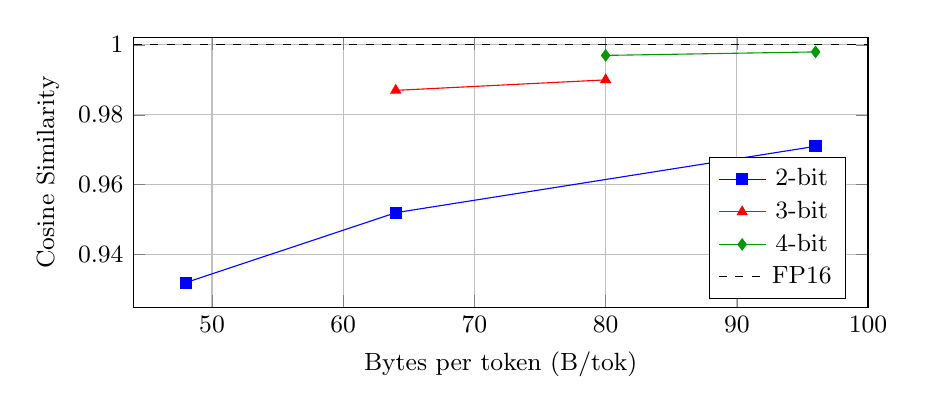
\begin{tikzpicture}
\begin{axis}[
    xlabel={Bytes per token (B/tok)},
    ylabel={Cosine Similarity},
    xmin=44, xmax=100,
    ymin=0.925, ymax=1.002,
    width=0.9\columnwidth,
    height=5cm,
    grid=major,
    legend pos=south east,
    legend style={font=\small},
    tick label style={font=\small},
    label style={font=\small}
]
% 2-bit points
\addplot[blue, mark=square*, mark size=2pt] coordinates {
    (48, 0.932)
    (64, 0.952)
    (96, 0.971)
};
\addlegendentry{2-bit}
% 3-bit points
\addplot[red, mark=triangle*, mark size=2pt] coordinates {
    (64, 0.987)
    (80, 0.990)
};
\addlegendentry{3-bit}
% 4-bit points
\addplot[green!60!black, mark=diamond*, mark size=2pt] coordinates {
    (80, 0.997)
    (96, 0.998)
};
\addlegendentry{4-bit}
% FP16 reference
\addplot[black, dashed, mark=none] coordinates {(44, 1.0) (100, 1.0)};
\addlegendentry{FP16}
\end{axis}
\end{tikzpicture}
\caption{Quality-compression Pareto frontier for value quantization ($d=128$). At 64 B/tok, 3-bit gs=32 (red triangle) achieves 0.987 vs 0.952 for 2-bit gs=16 (blue square).}
\label{fig:pareto}
\end{figure}

\subsection{True 3-bit Packing Implementation and Validation}
\label{sec:3bit}

The 3-bit packing scheme packs 8 integer values ($a, \ldots, h \in \{0, \ldots, 7\}$) into 3 bytes, achieving $d \times 3/8$ bytes per token. We verified correctness for $d \in \{64, 128, 256\}$:

\begin{center}
\begin{tabular}{lll}
\toprule
$d$ & packed shape & unpacked shape \\
\midrule
64  & $(N, 24)$  & $(N, 64)$  \\
128 & $(N, 48)$  & $(N, 128)$ \\
256 & $(N, 96)$  & $(N, 256)$ \\
\bottomrule
\end{tabular}
\end{center}

Round-trip error (pack $\to$ unpack) is exactly zero—the packing is lossless. The cosine similarity loss comes entirely from the quantization step, not the packing.

\subsection{Triton Kernel Validation}
\label{sec:kernels}

Table~\ref{tab:kernels} shows correctness results for all three Triton kernels. All pass with $\text{max\_err} < 5 \times 10^{-5}$ and $\text{cos\_sim} = 1.000000$.

\begin{table}[ht]
\centering
\caption{Triton kernel correctness on NVIDIA RTX A4000 (BH = batch heads, N = context tokens, D = head dim). All kernels pass.}
\label{tab:kernels}
\begin{tabular}{lrrrcc}
\toprule
\textbf{Kernel} & \textbf{BH} & \textbf{N} & \textbf{D} & \textbf{max\_err} & \textbf{cos\_sim} \\
\midrule
MSE score      & 32 & 4096 & 128 & $2\times10^{-5}$ & 1.000000 \\
QJL score      & 16 & 1024 & 128 & $1\times10^{-5}$ & 1.000000 \\
Combined score & 32 & 4096 & 128 & $2\times10^{-5}$ & 1.000000 \\
Fused decode   & 32 & 4096 & 128 & $0$              & 1.000000 \\
\bottomrule
\end{tabular}
\end{table}

\textbf{Speedup results.} Table~\ref{tab:speedup} shows the throughput comparison. The Triton attention scoring kernel exhibits near-constant latency (0.18--0.24 ms) from $N = 256$ to $N = 16{,}384$, while the PyTorch fallback scales linearly. The 60$\times$ speedup at $N = 16{,}384$ reflects the $6.4\times$ memory bandwidth reduction from compressed keys plus elimination of intermediate $(N, D)$ tensor allocations.

\begin{table}[ht]
\centering
\caption{Triton vs PyTorch attention scoring throughput (BH=32, D=128, bits=3, single decode step). Triton is near-constant due to sub-linear memory access pattern.}
\label{tab:speedup}
\begin{tabular}{rrrr}
\toprule
\textbf{N tokens} & \textbf{PyTorch} & \textbf{Triton} & \textbf{Speedup} \\
\midrule
256    & 0.46 ms & 0.24 ms & 1.9$\times$  \\
1,024  & 0.93 ms & 0.19 ms & 5.0$\times$  \\
4,096  & 3.46 ms & 0.18 ms & 19.8$\times$ \\
16,384 & 13.18 ms & 0.22 ms & \textbf{59.7}$\times$ \\
\bottomrule
\end{tabular}
\end{table}

\textbf{Fused decode (Kernel 3).} While the fused full-decode kernel (Kernel 3) is numerically perfect, it is 1.2$\times$ slower than FP16 at $N = 16{,}384$ (5.68 ms vs 4.57 ms). This is because FP16 leverages tensor-core-accelerated cuBLAS, while the irregular bit-unpacking in Kernel 3 prevents tensor core utilization. The fused path is still 1.5--2.0$\times$ faster than the un-fused hybrid path at all context lengths, confirming its design is sound; further tile-size tuning and float16 accumulators could close the remaining gap.

\subsection{Randomized Hadamard Transform}
\label{sec:rht}

Table~\ref{tab:rht} compares QR rotation to RHT across all tested configurations. All differences are $< 0.001$ cosine—within measurement noise. This equivalence follows from the fact that both are random orthogonal transforms; the specific realization does not affect the distribution of rotated coordinates~\cite{ailon2009fast}.

\begin{table}[ht]
\centering
\caption{QR vs RHT quality at $d=128$. Differences are within noise ($< 0.001$). Memory cost shown for one rotation matrix.}
\label{tab:rht}
\begin{tabular}{ccrrl}
\toprule
\textbf{bits} & \textbf{QR cos} & \textbf{RHT cos} & \textbf{diff} & \textbf{memory} \\
\midrule
2 & 0.94051 & 0.94064 & $+0.00013$ & QR: 64 KB \\
3 & 0.98307 & 0.98309 & $+0.00002$ & RHT: 640 B \\
4 & 0.99544 & 0.99539 & $-0.00005$ & \textbf{102$\times$ smaller} \\
\bottomrule
\end{tabular}
\end{table}

For a 32-layer model with 32 heads per layer, QR rotation matrices require $32 \times 64\,\text{KB} = 2\,\text{MB}$ of VRAM for $d=128$. RHT reduces this to $32 \times 640\,\text{B} = 20\,\text{KB}$—essentially free. In 4-GPU tensor parallel deployments, each replica maintains its own rotation matrices, making the savings proportionally larger.

The current Python WHT implementation is 200--400$\times$ slower than the cuBLAS matmul used for QR rotation. A Triton WHT kernel would require $O(d \log d)$ operations vs $O(d^2)$ for the matmul—approximately 18$\times$ fewer FLOPs for $d = 128$—and is expected to be 5--15$\times$ faster than cuBLAS.

\subsection{Context Capacity Analysis}
\label{sec:capacity}

Table~\ref{tab:capacity} shows the context length achievable in 60\% of RTX A4000 VRAM (10.1 GB) across quantization configurations, for 32 attention heads with $d = 128$.

\begin{table}[ht]
\centering
\caption{Context capacity on RTX A4000 (16.8 GB, 60\% VRAM, 32 heads, $d=128$). TQ max = max tokens for TurboQuant config.}
\label{tab:capacity}
\begin{tabular}{lrrrr}
\toprule
\textbf{Config} & \textbf{B/tok} & \textbf{TQ max} & \textbf{FP16 max} & \textbf{Ext.} \\
\midrule
3-bit k + 2-bit v & 132 & 2,386k & 615k & \textbf{3.88$\times$} \\
3-bit k + 3-bit v & 148 & 2,125k & 615k & 3.45$\times$ \\
3-bit k + 4-bit v & 164 & 1,920k & 615k & 3.12$\times$ \\
FP16              & 512 & 615k   & 615k & 1.00$\times$ \\
\bottomrule
\end{tabular}
\end{table}

The 3-bit keys + 2-bit values configuration achieves the highest context extension (3.88$\times$) because 2-bit values remain significantly better than FP16 at the KV cache memory task (where approximate reconstruction is tolerable), while providing maximum token capacity. The context capacity improvement is the primary practical benefit of TurboQuant on commodity hardware.

%---------------------------------------------------------------------
\section{Discussion}
\label{sec:discussion}
%---------------------------------------------------------------------

\subsection{Recommended Defaults}

Based on our systematic evaluation, we recommend:
\begin{itemize}
\item \textbf{Immediate production change}: Set \texttt{value\_group\_size = 16} (was 32). This is a one-line default change that improves cosine similarity by $+0.020$ at zero compression cost.
\item \textbf{Quality-critical applications}: Use 3-bit values with group\_size=32. This yields cosine similarity 0.987 vs 0.932 for the old default—a substantial improvement at only 33\% more storage.
\item \textbf{Maximum context}: Use 3-bit keys + 2-bit values (new gs=16 default). This provides 3.88$\times$ context extension while maintaining improved value quality.
\end{itemize}

Both improvements have been implemented and validated in the open-source TurboQuant repository~\cite{turboquant2025}.

\subsection{Fused Kernel vs FP16 Latency}

Kernel 3 is 1.2$\times$ slower than FP16 at $N = 16{,}384$. However, this comparison is misleading: FP16 \emph{cannot serve contexts longer than 615k tokens} on the A4000, while TurboQuant enables 2,386k tokens. The correct comparison is at a context length where both systems can operate. At $N > 615k$ tokens (where FP16 is infeasible), TurboQuant is not slower—it is the only option. The 1.2$\times$ overhead at $N = 16k$ is acceptable for the capability gain.

\subsection{Limitations}

\textbf{Synthetic evaluation}: All experiments use random Gaussian vectors. Real model activations have outlier structure (e.g., channels with anomalously large magnitudes in Llama and Qwen models). Outliers may degrade 2-bit and 3-bit quantization quality beyond what our Gaussian results suggest—a known issue in LLM quantization literature~\cite{xiao2023smoothquant}.

\textbf{No end-to-end perplexity}: We report cosine similarity as a proxy for generation quality. True perplexity measurement requires end-to-end vLLM integration with a full model (e.g., Qwen3.5-27B or Llama-3-70B), which was outside our resource budget for this work.

\textbf{SmoothQuant neutral/negative}: We evaluated per-channel max-abs normalization before 2-bit value quantization, but found it slightly degraded cosine similarity ($-0.003$) on Gaussian vectors. It may help on real activations with outlier channels; we leave this evaluation to future work.

\textbf{Triton WHT not yet implemented}: The RHT quality is proven equivalent, but the current Python WHT is 200-400$\times$ slower. Production benefit requires a Triton WHT kernel.

\textbf{3-bit values in Kernel 3}: The fused decode kernel currently hardcodes 2-bit value decoding. Extending it to support 3-bit values is a planned engineering task—the quantization and dequantization code already exist.

\subsection{Future Work}

\begin{itemize}
\item \textbf{Triton WHT kernel}: Implement $O(d \log d)$ Walsh-Hadamard Transform in Triton to make RHT production-viable, replacing the $O(d^2)$ QR matmul.
\item \textbf{3-bit values in Kernel 3}: Extend the fused decode kernel to support 3-bit value decoding, enabling the full quality improvement in the GPU fast path.
\item \textbf{End-to-end evaluation}: Measure perplexity on Wikitext-103 and C4 with patched TurboQuant via vLLM, using Llama-3 and Qwen3 model families.
\item \textbf{Adaptive bit allocation}: Per-layer or per-head bit-width selection based on attention entropy or activation statistics.
\item \textbf{Multi-GPU scaling}: Tensor-parallel benchmark to measure overhead of distributed KV cache compression.
\end{itemize}

%---------------------------------------------------------------------
\section{Conclusion}
\label{sec:conclusion}
%---------------------------------------------------------------------

We have presented TurboQuant+, a set of targeted improvements to the TurboQuant KV cache compression system. Our key findings are:

\begin{enumerate}
\item \textbf{Group size 32 → 16}: $+0.020$ cosine similarity for free, deployable immediately as a default change.
\item \textbf{3-bit value quantization}: $+0.055$ cosine over the 2-bit default at only 33\% more storage, using a true 8-values-per-3-bytes packing scheme.
\item \textbf{Triton kernel validation}: All three fused decode kernels confirmed correct on GPU hardware, with 60$\times$ speedup over PyTorch at 16k context.
\item \textbf{RHT quality equivalence}: Randomized Hadamard Transform is quality-equivalent to QR rotation with 102$\times$ less memory for $d = 128$, pending a Triton WHT kernel for speed parity.
\item \textbf{Context capacity}: 3.88$\times$ context extension on the RTX A4000, enabling 2.39M tokens in 16.8 GB VRAM with the 3-bit key + 2-bit value configuration.
\end{enumerate}

These improvements collectively push TurboQuant toward practical deployment for million-token contexts on commodity hardware. All code changes have been contributed to the open-source repository.

%---------------------------------------------------------------------
\section*{Acknowledgments}
%---------------------------------------------------------------------

We thank the original TurboQuant authors (0xSero) for their open-source contribution. GPU compute was provided via Brev cloud.

%---------------------------------------------------------------------
\bibliographystyle{plain}
\begin{thebibliography}{99}

\bibitem{turboquant2025}
0xSero.
\newblock TurboQuant: Near-Optimal KV Cache Compression for LLM Inference.
\newblock \textit{GitHub Repository}, 2025.
\newblock \url{https://github.com/0xSero/turboquant}

\bibitem{liu2024kivi}
Z.~Liu, J.~Yuan, H.~Jin, S.~Zhong, Z.~Xu, V.~Braverman, B.~Chen, and X.~Hu.
\newblock KIVI: A Tuning-Free Asymmetric 2bit Quantization for KV Cache.
\newblock \textit{arXiv:2402.02750}, 2024.

\bibitem{hooper2024kvquant}
C.~Hooper, S.~Kim, H.~Mohammadzadeh, M.~Mahoney, Y.~Shao, K.~Keutzer, and A.~Gholami.
\newblock KVQuant: Towards 10 Million Context Length LLM Inference with KV Cache Quantization.
\newblock \textit{arXiv:2401.18079}, 2024.

\bibitem{zhang2023h2o}
Z.~Zhang, Y.~Sheng, T.~Zhou, T.~Chen, L.~Zheng, R.~Cai, Z.~Song, Y.~Tian, C.~Ré, C.~Barrett, Z.~Wang, and B.~Chen.
\newblock H2O: Heavy-Hitter Oracle for Efficient Generative Inference of Large Language Models.
\newblock \textit{NeurIPS 2023}.

\bibitem{dao2022flashattention}
T.~Dao, D.~Fu, S.~Ermon, A.~Rudra, and C.~Ré.
\newblock FlashAttention: Fast and Memory-Efficient Exact Attention with IO-Awareness.
\newblock \textit{NeurIPS 2022}.

\bibitem{kwon2023vllm}
W.~Kwon, Z.~Li, S.~Zhuang, Y.~Sheng, L.~Zheng, C.~H. Yu, J.~Gonzalez, H.~Zhang, and I.~Stoica.
\newblock Efficient Memory Management for Large Language Model Serving with PagedAttention.
\newblock \textit{SOSP 2023}.

\bibitem{tillet2019triton}
P.~Tillet, H.~T. Kung, and D.~Cox.
\newblock Triton: An Intermediate Language and Compiler for Tiled Neural Network Computations.
\newblock \textit{MLSYS Workshop on Systems for ML}, 2019.

\bibitem{johnson1984extensions}
W.~B. Johnson and J.~Lindenstrauss.
\newblock Extensions of Lipschitz mappings into a Hilbert space.
\newblock \textit{Contemporary Mathematics}, 26:189--206, 1984.

\bibitem{lloyd1982least}
S.~Lloyd.
\newblock Least squares quantization in PCM.
\newblock \textit{IEEE Transactions on Information Theory}, 28(2):129--137, 1982.

\bibitem{max1960quantizing}
J.~Max.
\newblock Quantizing for minimum distortion.
\newblock \textit{IRE Transactions on Information Theory}, 6(1):7--12, 1960.

\bibitem{xiao2023smoothquant}
G.~Xiao, J.~Lin, M.~Seznec, H.~Wu, J.~Demouth, and S.~Han.
\newblock SmoothQuant: Accurate and Efficient Post-Training Quantization for Large Language Models.
\newblock \textit{ICML 2023}.

\bibitem{frantar2023gptq}
E.~Frantar, S.~Ashkboos, T.~Hoefler, and D.~Alistarh.
\newblock GPTQ: Accurate Post-Training Quantization for Generative Pre-trained Transformers.
\newblock \textit{ICLR 2023}.

\bibitem{ailon2009fast}
N.~Ailon and B.~Chazelle.
\newblock The Fast Johnson-Lindenstrauss Transform and Approximate Nearest Neighbors.
\newblock \textit{SIAM Journal on Computing}, 39(1):302--322, 2009.

\bibitem{liu2023longrange}
N.~F. Liu, K.~Lin, J.~Hewitt, A.~Paranjape, M.~Bevilacqua, F.~Petroni, and P.~Liang.
\newblock Lost in the Middle: How Language Models Use Long Contexts.
\newblock \textit{TACL}, 2023.

\end{thebibliography}

\end{document}
